\documentclass[a4paper]{article}
\usepackage[pdftex]{graphicx}
\usepackage[utf8]{inputenc}
\usepackage{enumerate}
\usepackage{siunitx}
\sisetup{locale=DE} 
\DeclareSIUnit \massunit {u}
\usepackage{icomma}
\usepackage{amssymb}
\hyphenation{Ver-ein-fach-ung}
\usepackage{tikz}
\usepackage{href-ul}
\hypersetup{
	colorlinks=true,
	linkcolor=blue,
	urlcolor=blue}
\usepackage{geometry}
\geometry{a4paper, top=15mm, left=15mm, right=15mm, bottom=15mm,
	headsep=10mm, footskip=12mm}

\begin{document}
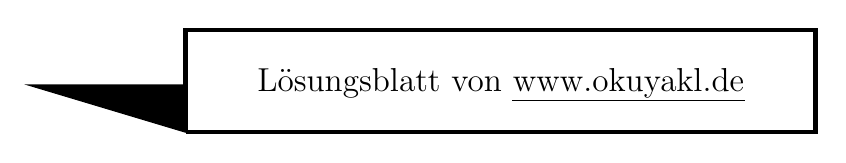
\begin{tikzpicture}(10,3)
	\draw[ultra thick](2,0) --(10,0) -- (10,1.3) --(2,1.3) -- (2,0);
	\draw[fill=black](2,0)-- (0,.6) -- (2,.6) -- (2,0);
	\node at (6,.6) {\large Lösungsblatt von \href{https://www.okuyakl.de}{www.okuyakl.de}};
\end{tikzpicture}
\vspace{0.5 cm}


\noindent{\bf Aufgabe 1.}\\
Die Summe der Einzelimpulse, der Gesamtimpuls, ist vor und nach dem Stoß gleich. Hierbei spielt es keine Rolle, ob der Stoß elastisch oder unelastisch erfolgt.
\vspace{0.5 cm}

\noindent{\bf Aufgabe 2. a)}\\
Es gilt für den unelastischen Stoß folgende Beziehung. Hierbei sei $v_1$ und $m_1$ die Geschwindigkeit in $\SI{}{\meter\over\second}$ und die Masse des Kleinbusses, $v_2$ und $m_2$ die Geschwindigkeit und die Masse des Kleinwagens. Beide Fahrzeuge bewegen sich nach dem Stoß mit der gleichen Geschwindigkeit $u$ gemeinsam weiter:

$$
\renewcommand{\arraystretch}{2}
\begin{array}{rcll}
m_1 v_1 + m_2 v_2 &=&(m_1 + m_2)\cdot u &|:(m_1 + m_2) \\
u &=& {m_1 v_1 + m_2 v_2 \over  m_1 + m_2} \\
u &=& {\SI{1700}{\kilogram} \cdot  \SI{15}{\meter\over\second} + \SI{650}{\kilogram} \cdot (\SI{-10}{\meter\over\second})\over \SI{1700}{\kilogram} +  \SI{650}{\kilogram}} & = \SI{8,1}{\meter\over\second}
\end{array}
$$ 
$u$ besitzt das gleiche Vorzeichen wie $v_1~\Rightarrow$ Beide Fahrzeuge bewegen sich mit $u=\SI{8,1}{\meter\over\second} = \SI{29}{\kilo\meter\over\hour}$ in Fahrtrichtung des Kleinbusses weiter.
\vspace{0.5 cm}

\noindent{\bf Aufgabe 2. b)}\\
Wir vergleichen die Gesamtenergie vor dem Stoß $E_{kin,v}$ mit der nach dem Stoß $E_{kin,n}$. Die kinetische Energie  nach einem elastischen Stoß wird kleiner. Die Differenz wird in Verformungsarbeit und innere Energie $E_{v,i}$ umgewandelt.
$$
\renewcommand{\arraystretch}{2}
\begin{array}{rcl}
E_{v,i} & = & \Delta E_{kin}  = E_{kin,v} - E_{kin,n} \\
        & = & {1 \over 2}m_1 \cdot v_1^2 + {1 \over 2}m_2 \cdot v_2^2
        - {1 \over 2}\cdot (m_1+m_2) \cdot u^2  \\
        & = & {1 \over 2}\cdot \SI{1700}{\kilogram} \cdot (\SI{15}{\meter\over\second})^2 + {1 \over 2}\cdot\SI{650}{\kilogram} \cdot (\SI{10}{\meter\over\second})^2
        - {1 \over 2}\cdot (\SI{1700}{\kilogram} + \SI{650}{\kilogram}) \cdot (\SI{8,1}{\meter\over\second})^2\\
        & = & \SI{223750}{\joule} - \SI{77092}{\joule}\\
        & = & \SI{146658}{\joule} \approx \SI{150}{\kilo\joule} 
\end{array}
$$
Der prozentuale Anteil $x \%$ der Verformungsarbeit an der Gesamtenergie ist:
$$ x\% = {E_{v,i}\over E_{kin,v}}\cdot 100\%= 66\%$$
\vspace{0.5 cm}

\noindent{\bf Aufgabe 3. a)}\\
Kraft $F$ ist gleich Impulsänderung $\Delta p $ mit der Zeit:
$$F = {\Delta p  \over \Delta t} \qquad (*) $$
Impuls ist gleich Masse mal Geschwindigkeit; hier verändert sich die Masse der Rakete, die Geschwindigkeit der Verbrennungsgase bleibt konstant, also ist Impulsänderung hier gleich Massenänderung $\Delta m$ im Zeitintervall $ \Delta t = \SI{1}{\second}$ mal Geschwindigkeit. Aus $(*)$ wird dann:
$$F= {\Delta m \cdot v  \over \Delta t} \Leftrightarrow {\Delta m \over \Delta t}= {F \over v}$$
$$ {\Delta m \over \Delta t} = {\SI{2,0e5}{\newton} \over  \SI{2000}{\meter\over\second}} = \SI{100}{kg \over s}$$
Einheitencheck:
$$ {\SI{}{\newton\over{\meter\over\second}}}= \SI{}{\kilogram\cdot {\meter\over{\second^2}} \over {\meter\over\second}} = \SI{}{\kilogram\over \second}$$
Pro Sekunde mussten $\SI{100}{\kilogram}$ Treibstoff verbrannt werden. 
\vspace{0.5 cm}

\noindent{\bf Aufgabe 3. b)}\\
Für die beschleunigende Kraft gilt, dass sie gleich der Differenz der Schub- mit der Gewichtskraft ist. Nach dem Trägheitssatz erhalten wir für die Beschleunigung $a$:
$$
\renewcommand{\arraystretch}{2}
\begin{array}{rcll}
F_a &=& F_{Schub}-F_G &\stackrel{!}{=} m \cdot a\\
  a &=& {F_{Schub}-F_G \over m} & = {\SI{2,0e5}{\newton} - \SI{10000}{\kilogram}\cdot  \SI{9,81}{\meter\over{\second^2}} \over \SI{10000}{\kilogram} }\\
  a &=&  \SI{10}{\meter \over {\second^2}}
\end{array}
$$
\vspace{0.5 cm}

\noindent{\bf Aufgabe 4. a)}\\
Impuls vor dem Zerfall = Impuls nach dem Zerfall:
$$
\renewcommand{\arraystretch}{2}
\begin{array}{rcll}
 0 &=& m_1v_1 + m_2v_2 \\
 v_1 &=& - {m_2 \over m_1}v_2 \\
 v_1 &=& -{\SI{4}{\massunit} \over \SI{234}{\massunit}} \cdot\SI{1,4e7}{\meter\over \second}\\
 v_1 &=& \SI{-2,4e5}{\meter\over \second}
\end{array}
$$
\vspace{0.5 cm}

\noindent{\bf Aufgabe 4. b)}\\
Das Verhältnis beider kinetischer Energien kann man berechnen, ohne sie einzeln genau zu bestimmen:
$$
{E_{kin1}\over E_{kin2}}= {{1 \over 2}m_1v_1^2 \over {1 \over 2} m_2v_2^2} = { \SI{234}{\massunit} \cdot (\SI{2,4e5}{\meter\over \second})^2 \over \SI{4}{\massunit}\cdot (\SI{1,4e7}{\meter\over\second})^2}=0,0172 \approx 1 : 58$$
\vspace{0.5 cm}

\noindent{\bf Aufgabe 5.}\\
Der Impuls des Asteroiden betrug:
$$p=m_1v_1=\SI{7,0e13}{\kilogram} \cdot \SI{20e3}{\meter\over \second} = \SI{1,4e18}{\newton\cdot\second}$$
Die Erde erhält dadurch eine Geschwindigkeitsänderung von:
$$
\renewcommand{\arraystretch}{2}
\begin{array}{rcll}
 m_1v_1 &=& (m_1+m_2)u \\
 u &=& {m_1v_1 \over m_1+m_2}\\
 u &=& {\SI{1,4e18}{\newton\cdot\second}\over\SI{5,97e24}{\kilogram} +\SI{7,0e13}{\kilogram}}\\
 u &=& \SI{2,3e-7}{\meter\over \second}
\end{array}
$$ 
Die Geschwindigkeit nach dem Stoß ist minimal, die Erde bleibt in ihrer Bahn.
(Bahngeschwindigkeit der Erde relativ zur Sonne: $v \approx \SI{30}{\kilo\meter\over \second}$)
\vspace{0.5 cm}

\noindent{\bf Aufgabe 6. a)}\\
Die Geschwindigkeit der Masse $m_2$ vor der Impulsübertragung ist:
$$v_2 = \sqrt{2gh} = \sqrt{2\cdot \SI{9,81}{\meter \over {\second^2}} \cdot \SI{0,30}{\meter}}=\SI{2,4}{\meter\over \second}$$
Die Masse $m_1$ bekommt dann die Geschwindigkeit:
$$
\renewcommand{\arraystretch}{2}
\begin{array}{rcll}
 m_2v_2 &=& (m_1+m_2)u \\
  u &=& {m_2v_2 \over m_1 + m_2} \\
  u &=& \SI{1,1}{\meter\over\second}
\end{array}
$$
\vspace{0.5 cm}

\noindent{\bf Aufgabe 6. b)}\\
Die potentielle Energie, die beim Aufsteigen der Masse $m_1$ gewonnen wird, ist:
$$E_{pot}=E_{pot1}-E_{pot2} = (m_1-m_2)gh$$
\vspace{0.5 cm}

\noindent
\begin{minipage}{0.5\textwidth}
Wir setzen gleich mit der kinetischen Energie des Systems:
$$
\renewcommand{\arraystretch}{2}
\begin{array}{rcll}
E_{pot}&=&E_{kin} \\
(m_1-m_2)gh &=& {1 \over 2}(m_1+m_2)u^2 \\
h &=& {(m_1 +m_2)u^2 \over 2 (m_1-m_2)g} \\
h &=& \SI{0,56}{\meter}
\end{array}
$$ 	
\end{minipage}
\hfill
\begin{minipage}{0.5\textwidth}
\begin{center}
	\includegraphics[width=7 cm]{../../viecher/endcomic.pdf}
	
	Hier geht es zurück zum \href{https://www.okuyakl.de/phys/p10impL136/aa136.pdf}{Aufgabenblatt}
\end{center}

\end{minipage}


%Ende
\end{document}